% !TeX encoding = UTF-8
% !TeX spellcheck = es_ES

\section{Ejemplo de la ejecución}

Cuando el programa se ejecuta se siguen los pasos descritos en \textit{Explicación del programa} en el mismo orden que lo expuesto. Se empieza con distribuciones de tipo T-Student y cuando se llega a $k = 5$ ya pasamos a utilizar distribuciones normales. El programa se ejecuta hasta que $k = 6$ (inclusive) ya que en ese momento el p-valor es igual a $0.03858$ el cual es superior a $0.01$. Da como resultado una hipótesis de $70.23559$ con media $68.64111$. Los gráficos resultantes y mensajes de consola están en la siguiente página.

\begin{figure}[h]
	\begin{subfigure}{0.499\textwidth}
		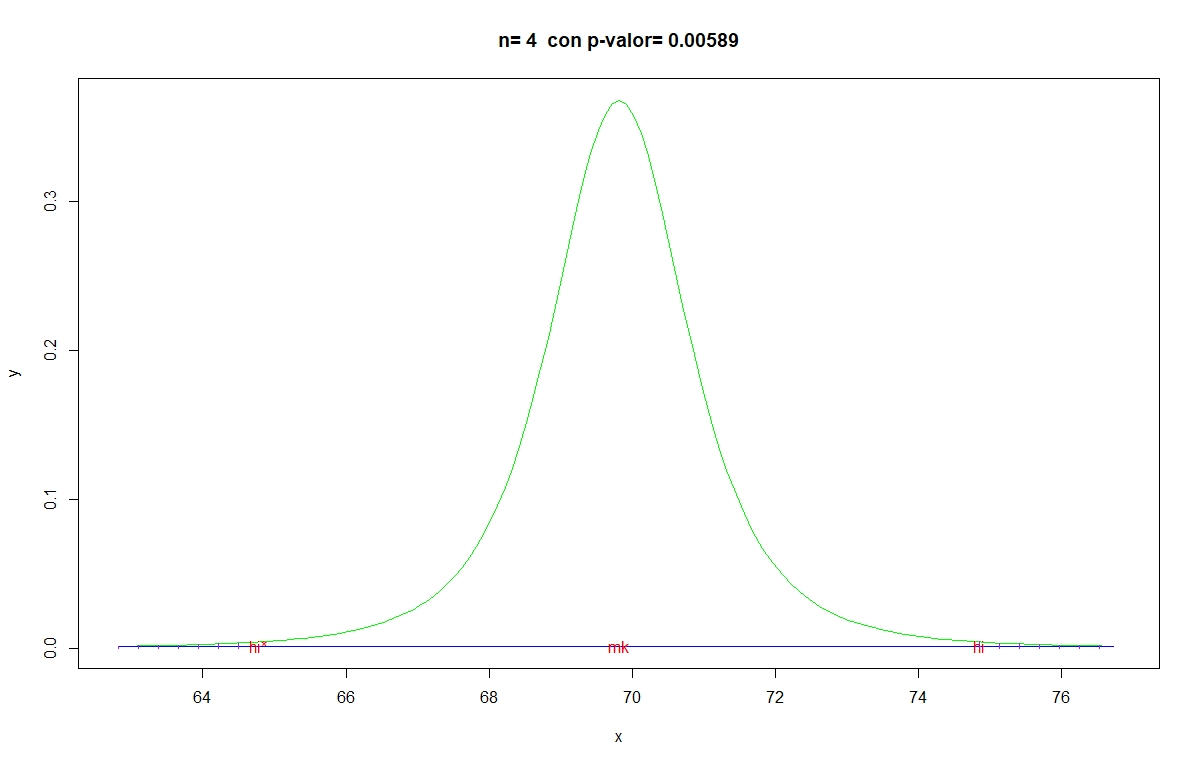
\includegraphics[width=\linewidth]{assets/ejemplo-4.jpeg}
		\caption{Mantenemos la hipótesis aumentando la muestra.}
		\label{fig:subim5}
	\end{subfigure}
	\begin{subfigure}{0.499\textwidth}
		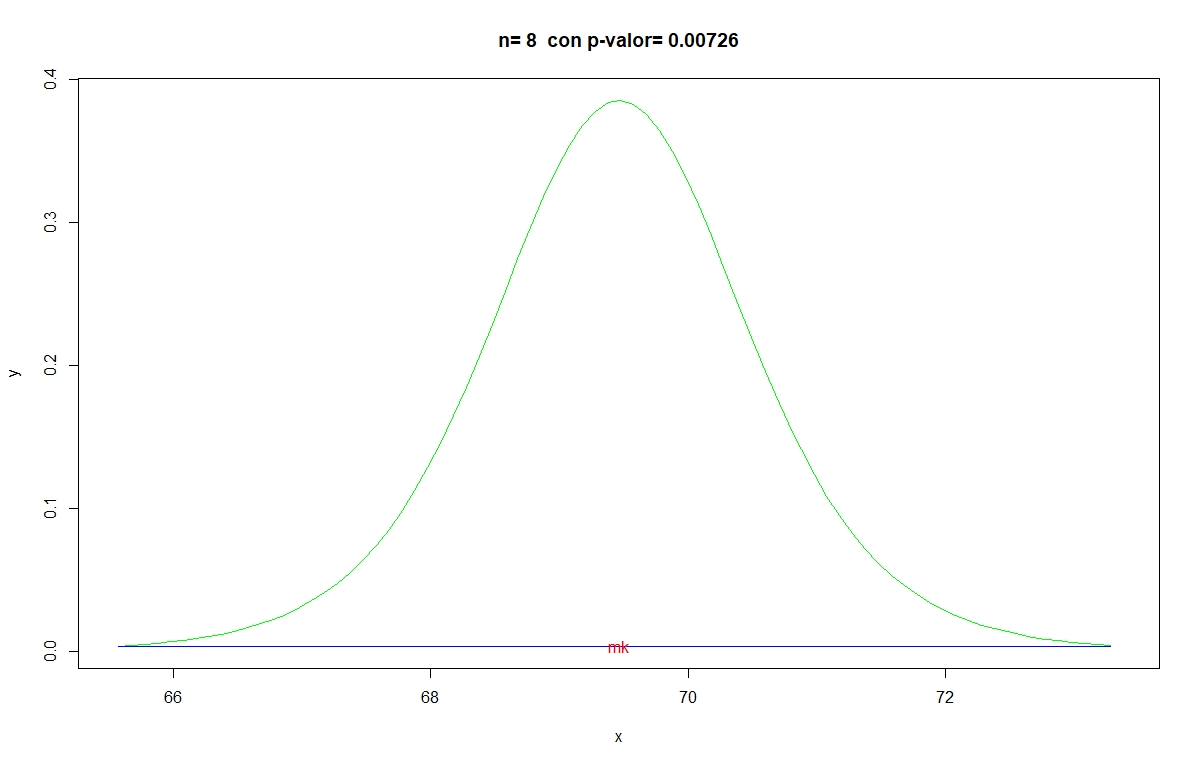
\includegraphics[width=\linewidth]{assets/ejemplo-8.jpeg}
		\caption{Mantenemos la hipótesis aumentando la muestra.}
		\label{fig:subim6}
	\end{subfigure}
	\begin{subfigure}{0.499\textwidth}
		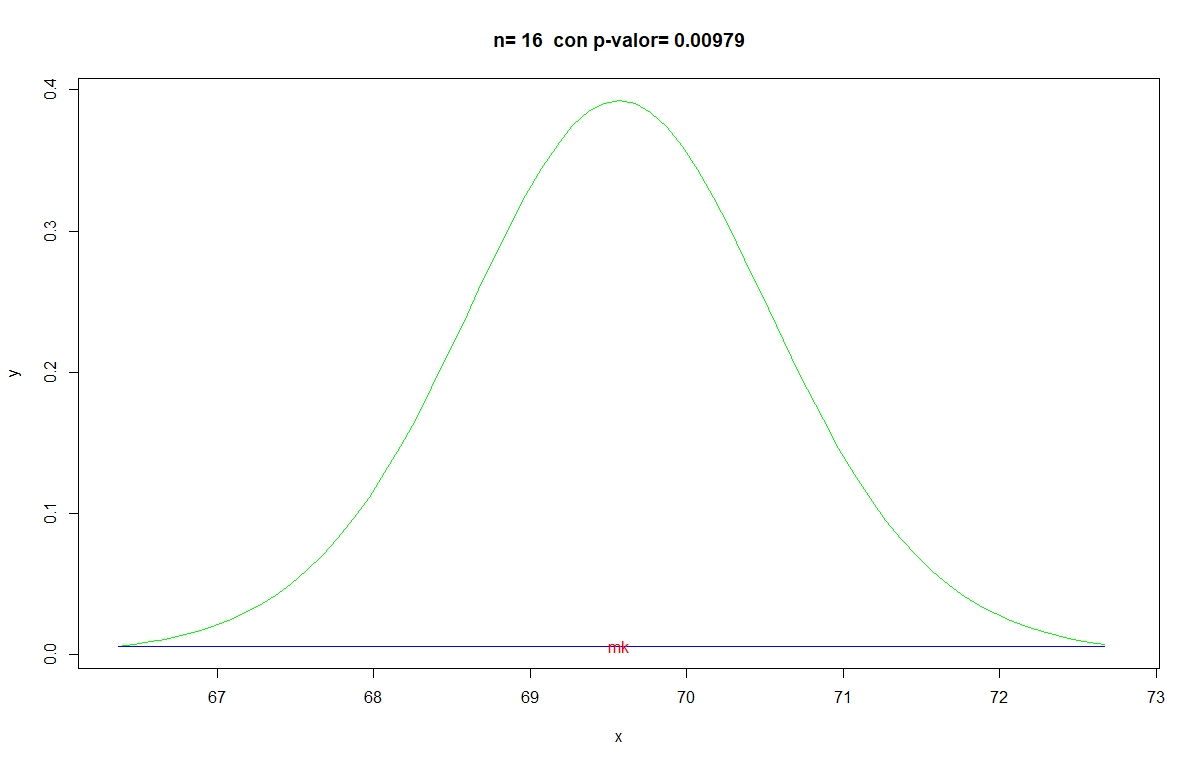
\includegraphics[width=\linewidth]{assets/ejemplo-16.jpeg}
		\caption{Mantenemos la hipótesis aumentando la muestra.}
		\label{fig:subim7}
	\end{subfigure}
	\begin{subfigure}{0.499\textwidth}
		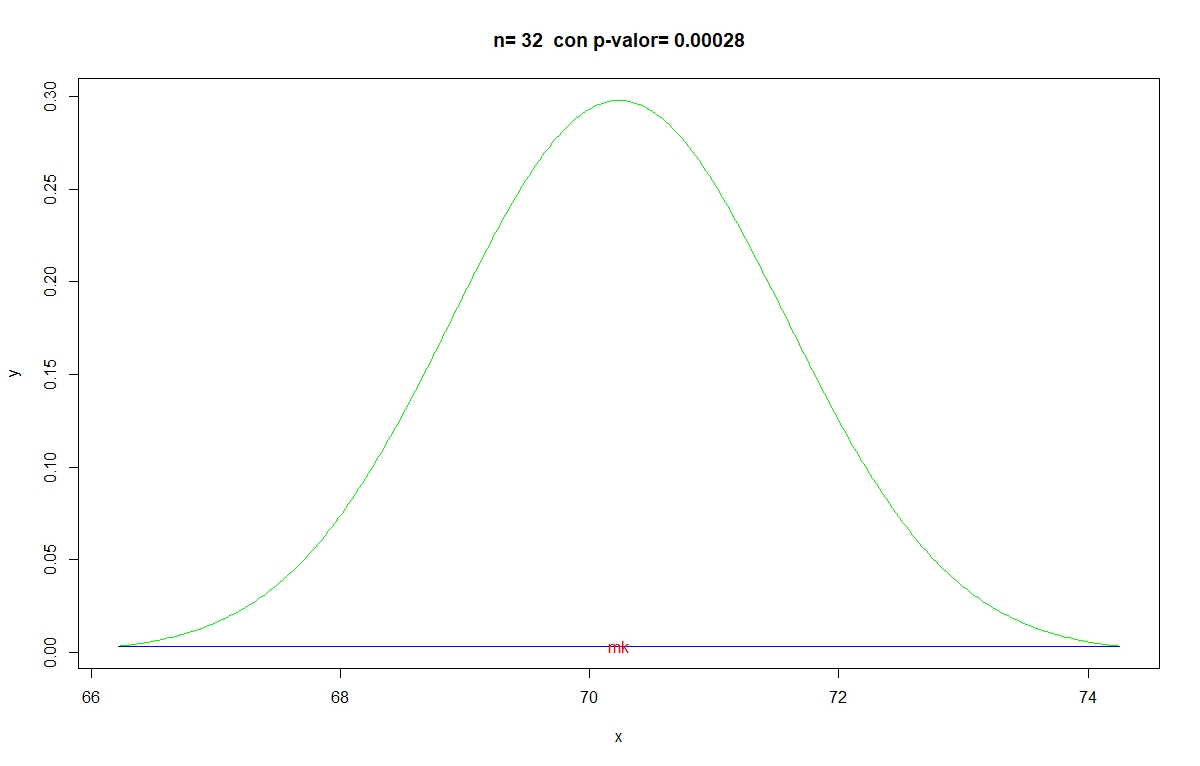
\includegraphics[width=\linewidth]{assets/ejemplo-32.jpeg}
		\caption{Rechazamos la hipótesis y la cambiamos mientras aumentamos la muestra.}
		\label{fig:subim8}
	\end{subfigure}
	\begin{subfigure}{0.499\textwidth}
		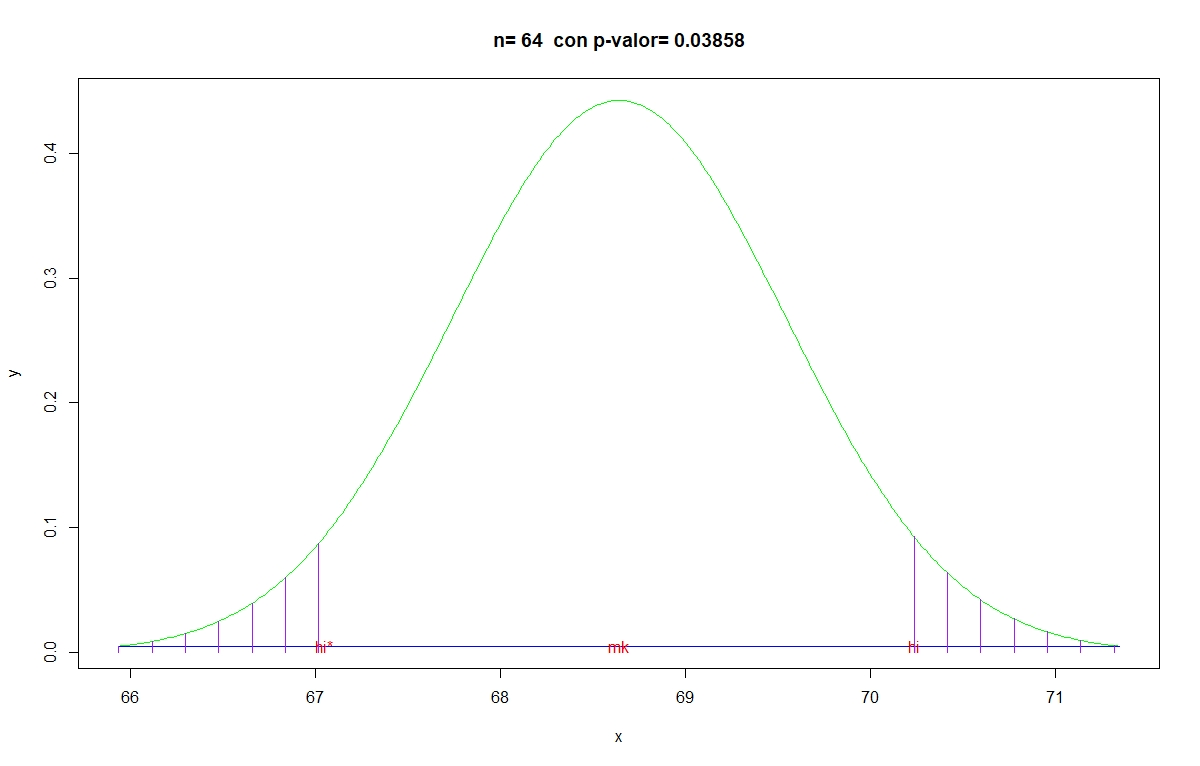
\includegraphics[width=\linewidth]{assets/ejemplo-64.jpeg}
		\caption{Aceptamos la hipótesis 70.23559 (media: 68.64111) debido a que  0.03858 es mayor que 0.01.}
		\label{fig:subim9}
	\end{subfigure}
	\caption{Resultados de la ejecución del programa}
	\label{fig:image3}
\end{figure}